\subsection{Ablation Studies}
\label{sec:ablation-studies}

We evaluate four controlled ablations to isolate the contribution of uncertainty routing, retrieved report evidence, and guarded LLM review. The complete pipeline is reported separately as Experiment~6 in Section~4.2. The test cohort, RAD-DINO checkpoint, label-specific operating thresholds, gray-zone margin, and Judge policy are held fixed as specified in Section~4.1. Table~\ref{tab:ablation-configurations} summarizes the enabled components.

\begin{table}[H]
\centering
\caption{Components enabled in the four ablation configurations. ``Gray $\rightarrow$ uncertain'' replaces every gray-zone prediction with an uncertain status without using retrieved evidence.}
\label{tab:ablation-configurations}
\resizebox{\columnwidth}{!}{%
\begin{tabular}{cllll}
\toprule
Exp. & Retrieval & Label fusion & LLM review & Evidence verification \\
\midrule
1 & No & None & None & None \\
2 & No & Gray $\rightarrow$ uncertain & None & None \\
3 & Yes & Deterministic & None & None \\
4 & Yes & Deterministic & Llama 3.1 8B & None \\
\bottomrule
\end{tabular}%
}
\end{table}

\subsubsection{Experiment 1: Vision-Only Baseline}

The first configuration evaluates the fine-tuned RAD-DINO classifier without retrieval, label fusion, or evidence verification. The checkpoint selected at epoch 2 achieved a validation macro-F1 of $0.5957$, macro-AUROC of $0.8458$, and macro average precision of $0.5935$. Training stopped after epoch 7 because validation macro-F1 did not improve for five consecutive epochs. On the held-out test cohort, the resulting vision-only predictions achieved macro precision $0.9108$, macro recall $0.5695$, and macro-F1 $0.6971$; the corresponding micro-F1 was $0.7042$. The gap between precision and recall shows that the baseline is conservative: its positive predictions are generally precise, but it fails to recover a substantial fraction of supervised-positive findings.

Within the frozen gray-zone scope, macro-F1 decreases to $0.6310$ and macro recall to $0.5090$, compared with macro precision of $0.8748$. This reduction confirms that threshold-adjacent decisions are materially more difficult than the complete test set and establishes the subset on which downstream intervention is evaluated. Figure~\ref{fig:vision-label-f1} reports the corresponding label-wise vision-only F1 values.

\begin{figure}[H]
\centering
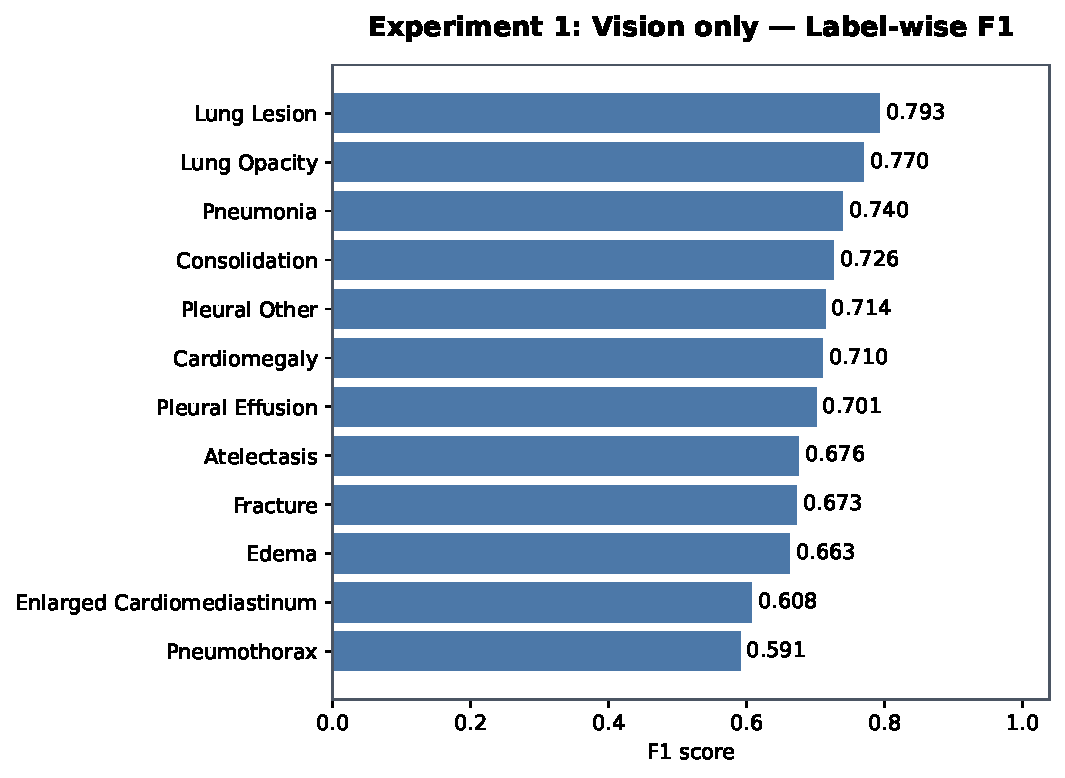
\includegraphics[width=\columnwidth]{v2/experiments/visualizations_exp01_exp06/paper_figures/exp01_label_f1.pdf}
\caption{Per-label F1 of the vision-only RAD-DINO baseline on Judge-scoreable test cells.}
\label{fig:vision-label-f1}
\end{figure}

\subsubsection{Experiment 2: Gray-Zone Abstention without Retrieval}

The second configuration tests whether uncertainty routing alone is sufficient to improve performance. All 1,812 labels in the frozen gray-zone mask are changed to \texttt{uncertain}, while the remaining 9,060 study--label decisions retain their vision-only status. This operation increases full-test macro precision from $0.9108$ to $0.9241$, but reduces macro recall from $0.5695$ to $0.4619$. Consequently, macro-F1 falls by $0.0845$, from $0.6971$ to $0.6126$, and micro-F1 falls from $0.7042$ to $0.6240$.

No gray-zone label remains predicted as present or absent after this transformation. Gray-zone precision and F1 are therefore undefined, while recall is $0$ under the Judge policy because a ground-truth-positive label predicted as uncertain is recorded as a missed positive. The result demonstrates that routing uncertainty without supplying additional evidence is excessively conservative: it removes some false positives, but the associated loss of true positives is substantially larger.

\subsubsection{Experiment 3: Deterministic Retrieval-Grounded Fusion}

The third configuration adds image-to-report retrieval and deterministic gray-zone fusion, without either LLM. Fusion changes 390 of the 1,812 routed study--label decisions: 374 absent-to-present promotions and 16 demotions from a vision-positive status. Full-test macro recall increases from $0.5695$ to $0.6051$, while macro precision remains effectively stable ($0.9108$ versus $0.9117$). Macro-F1 consequently increases by $0.0275$ to $0.7246$, and micro-F1 increases by $0.0341$ to $0.7383$.

The effect is concentrated in the region where intervention is permitted. Gray-zone macro-F1 increases from $0.6310$ to $0.7613$, and gray-zone micro-F1 increases from $0.6417$ to $0.8041$. Gray-zone recall rises by $0.1860$, from $0.5090$ to $0.6950$, while macro precision changes by only $+0.0025$. The largest useful promotion effects occur for Pleural Effusion, Lung Opacity, Edema, and Atelectasis, which gain 16, 13, 10, and 7 true positives, respectively, with at most one additional false positive per label. Pneumothorax is the principal adverse case: its fusion changes remove three false positives but also lose one true positive. These results identify retrieved report evidence, rather than uncertainty routing by itself, as the primary source of the predictive improvement.

\subsubsection{Experiment 4: Guarded LLM Fusion Review}

This configuration places an LLM reviewer after deterministic fusion while keeping evidence verification disabled. The label-fusion review uses Llama 3.1 8B \cite{grattafiori2024llama3}. The run requested reviews for 264 studies, of which 261 calls succeeded, and produced 372 label-level reviews. Although the run attains macro-F1 $0.7257$, its finalized labels do not differ from the deterministic proposals generated within that run. The $0.0011$ difference relative to Experiment 3 must therefore not be attributed to LLM correction; it results from rerunning the upstream vision and retrieval path, which produced 392 rather than 390 deterministic changes.

The guarded reviewer provides structured scrutiny of proposed updates but does not establish an additional scored predictive gain in this ablation. This is consistent with the intentionally restrictive authority assigned to the first LLM: malformed, weakly supported, or policy-inconsistent non-keep actions revert to the deterministic result.

\begin{table}[H]
\centering
\caption{Full-test Judge results for the four ablation configurations. All values are computed on the same 906 studies and 12-label output space.}
\label{tab:ablation-full-results}
\resizebox{\columnwidth}{!}{%
\begin{tabular}{clrrrrr}
\toprule
Exp. & Configuration & Macro P & Macro R & Macro F1 & Micro F1 & Coverage \\
\midrule
1 & Vision only & 0.9108 & 0.5695 & 0.6971 & 0.7042 & 0.1494 \\
2 & No-retrieval abstention & 0.9241 & 0.4619 & 0.6126 & 0.6240 & 0.1428 \\
3 & Deterministic retrieval fusion & 0.9117 & 0.6051 & 0.7246 & 0.7383 & 0.1492 \\
4 & Llama fusion review & 0.9117 & 0.6064 & 0.7257 & 0.7389 & 0.1491 \\
\bottomrule
\end{tabular}%
}
\end{table}

Overall, the ablations show that indiscriminate gray-zone abstention raises precision at an unacceptable recall cost, whereas retrieval-grounded deterministic fusion improves recall and F1 while preserving precision. Guarded LLM fusion review does not measurably improve scored labels beyond deterministic fusion in these runs; its role in the complete pipeline is therefore interpreted as constrained review and evidence characterization rather than as an additional source of predictive accuracy.
